\documentclass[8pt]{beamer}

\usetheme{metropolis}

\usepackage{pgfplots}
\usepackage{varwidth}
\usepackage{xcolor}

\usetikzlibrary{calc}

\date{19.01.23}
\title{Introduction to Machine Learning}
\subtitle{Image recognition in Python and Tensorflow}
\author{Esten H. Leonardsen and Martin Hovin}

\titlegraphic{
	\centering
}

\colorlet{model1}{red}
\colorlet{model2}{green}
\colorlet{model3}{orange}

\begin{document}
	\begin{frame}
		\maketitle
	\end{frame}

	\begin{frame}{Introduction} % Speakers
		\centering
		\vfill
		\begin{tikzpicture}
			\node[] (esten) at (0, 0) {
				\includegraphics[width=2cm]{data/esten.jpg}
			};
			\node[] (martin) at (0, -3) {
				\includegraphics[width=2cm]{data/martin.png}
			};
			\node[align=left, anchor=west] at (esten.east) {
				\textbf{Esten H. Leonardsen}\\
				(UiO and Biometrical AS)\\
				\underline{Interests:}\\
				- Talking about esoteric theory\\
				- Making deep learning tutorials
			};
			\node[align=left, anchor=west] at (martin.east) {
				\textbf{Martin Hovin}\\
				(Biometrical AS)\\
				\underline{Interests:}\\
				- Installing tensorflow\\
				- Debugging Estens code
			};
		\end{tikzpicture}
		\vfill
	\end{frame}

	\begin{frame}{Introduction} % Learning goals
		\vfill
		Theory session:
		\begin{itemize}
			\item What is a statistical learning model?
			\item What is a loss function?
			\item How do we train a statistical learning model?
			\item How does a (deep) neural network work?
			\item What operations does a convolutional neural network use?
			\item What is transfer learning?
			\item What is overfitting?
			\item How do we combat it?
		\end{itemize}
		Practical session:
		\begin{enumerate}
			\item Set up a Python-environment containing Tensorflow
			\item Use a pretrained convolutional neural network to predict
			\item Fit a flower classifier using transfer learning
			\item Improve the flower classifier
		\end{enumerate}
		\vfill
	\end{frame}

	\begin{frame}{Introduction} % Motivation: Brain classification
	\end{frame}

	\begin{frame}{Introduction} % Motivation: Biometrical
	\end{frame}

	\begin{frame}{Introduction} % Motivation: Gjensidige
	\end{frame}

	\begin{frame}{Introduction} % Motivation: Segmentation
	\end{frame}

	\begin{frame}{Introduction} % Motivation: Imagen
		\centering
		\vfill
		\includegraphics[width=7cm]{data/dog-in-sushihouse.png}
		\vfill
	\end{frame}

	\begin{frame}{Statistical learning models} % Finn.no data
		\centering
		\vfill
		\begin{tikzpicture}
			\node[draw=black, inner sep=0pt] at (0, 0) {
				\includegraphics[height=7cm]{data/finn.png}
			};
		\end{tikzpicture}
		\vfill
	\end{frame}

	\begin{frame}{Statistical learning models} % Dataset
		\centering
		\vfill
		\begin{table}
			\begin{tabular}{|c|c|}
				\hline
				\textbf{$m^2$}&\textbf{Price}\\
				\hline
				72&5.127.379\\
				\hline
				50&4.552.170\\
				\hline
				45&4.486.654\\
				\hline
				62&5.709.276\\
				\hline
				53&4.634.912\\
				\hline
				81&8.388.570\\
				\hline
				44&4.828.170\\
				\hline
				78&7.557.770\\
				\hline
				37&4.016.520\\
				\hline
				73&6.572.351\\
				\hline
			\end{tabular}
		\end{table}
		\vfill
	\end{frame}

	\begin{frame}{Statistical learning models} % General Model
		\vfill
		\begin{tikzpicture}
			\begin{axis}[
				xlabel=$m^2$,
				ylabel=NOK,
				ytick={4000000, 5000000, 6000000, 7000000, 8000000},
				yticklabels={4M, 5M, 6M, 7M, 8M},
				scaled y ticks=false,
				xtick pos=bottom,
				ytick pos=left,
				xmin=30,
				xmax=90,,
				ymin=3500000,
				ymax=8800000
			]
				\addplot[
					only marks,
					mark size=3pt,
					mark options={draw=black, fill=cyan}
				] coordinates {
					(72, 5127379)
					(50, 4552170)
					(45, 4486654)
					(62, 5709276)
					(53, 4634912)
					(81, 8388570)
					(44, 4828170)
					(78, 7557770)
					(37, 4016520)
					(73, 6572351)
				};

				\newcommand{\loss}[2]{
					\addplot[dashed] coordinates {
						(####1, 3500000 + ####1 * 30000)
						(####1, ####2)
					};
				}

				\coordinate (center) at (axis cs: 60, 3500000);
			\end{axis}
			\node[anchor=north,align=center] (m1) at ($ (center) - (0, 1) $) {
				$\hat{y}=f(x)$
			};

			\node[] at ($ (center) - (5.3, 1.8) $) {};
			\node[] at ($ (center) + (5.3, 5.8) $) {};
		\end{tikzpicture}
		\vfill
	\end{frame}

	\begin{frame}{Statistical learning models} % Linear model
		\vfill
		\begin{tikzpicture}
			\begin{axis}[
				xlabel=$m^2$,
				ylabel=NOK,
				ytick={4000000, 5000000, 6000000, 7000000, 8000000},
				yticklabels={4M, 5M, 6M, 7M, 8M},
				scaled y ticks=false,
				xtick pos=bottom,
				ytick pos=left,
				xmin=30,
				xmax=90,,
				ymin=3500000,
				ymax=8800000
			]
				\addplot[
					only marks,
					mark size=3pt,
					mark options={draw=black, fill=cyan}
				] coordinates {
					(72, 5127379)
					(50, 4552170)
					(45, 4486654)
					(62, 5709276)
					(53, 4634912)
					(81, 8388570)
					(44, 4828170)
					(78, 7557770)
					(37, 4016520)
					(73, 6572351)
				};

				\newcommand{\loss}[2]{
					\addplot[dashed] coordinates {
						(####1, 3500000 + ####1 * 30000)
						(####1, ####2)
					};
				}

				\coordinate (center) at (axis cs: 60, 3500000);
			\end{axis}
			\node[anchor=north,align=center] (m1) at ($ (center) - (0, 1) $) {
				$\hat{y}=Wx+b$
			};

			\node[] at ($ (center) - (5.3, 1.8) $) {};
			\node[] at ($ (center) + (5.3, 5.8) $) {};
		\end{tikzpicture}
		\vfill
	\end{frame}

	\begin{frame}{Statistical learning models} % Concrete model
		\vfill
		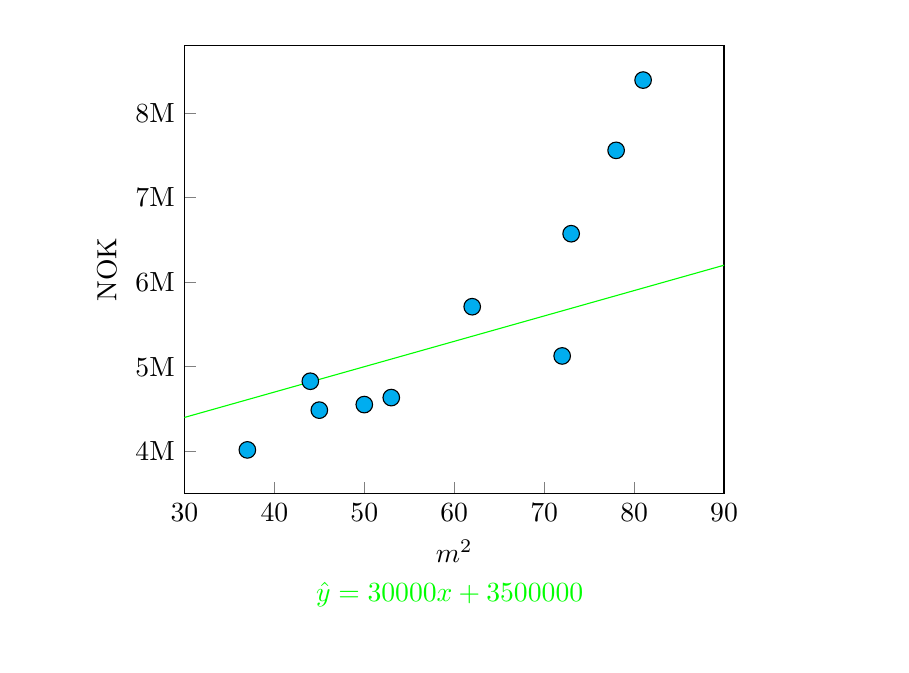
\begin{tikzpicture}
			\begin{axis}[
				xlabel=$m^2$,
				ylabel=NOK,
				ytick={4000000, 5000000, 6000000, 7000000, 8000000},
				yticklabels={4M, 5M, 6M, 7M, 8M},
				scaled y ticks=false,
				xtick pos=bottom,
				ytick pos=left,
				xmin=30,
				xmax=90,,
				ymin=3500000,
				ymax=8800000
			]
				\addplot[
					only marks,
					mark size=3pt,
					mark options={draw=black, fill=cyan}
				] coordinates {
					(72, 5127379)
					(50, 4552170)
					(45, 4486654)
					(62, 5709276)
					(53, 4634912)
					(81, 8388570)
					(44, 4828170)
					(78, 7557770)
					(37, 4016520)
					(73, 6572351)
				};
				\addplot[model2] coordinates {
					(0, 3500000)
					(100, 6500000)
				};

				\newcommand{\loss}[2]{
					\addplot[dashed] coordinates {
						(####1, 3500000 + ####1 * 30000)
						(####1, ####2)
					};
				}

				\coordinate (center) at (axis cs: 60, 3500000);
			\end{axis}
			\node[anchor=north,align=center, text=model2] (m1) at ($ (center) - (0, 1) $) {
				$\hat{y}=30000x + 3500000$
			};

			\node[] at ($ (center) - (5.3, 1.8) $) {};
			\node[] at ($ (center) + (5.3, 5.8) $) {};
		\end{tikzpicture}
		\vfill
	\end{frame}

	\begin{frame}{Statistical learning models} % Alternative models
		\vfill
		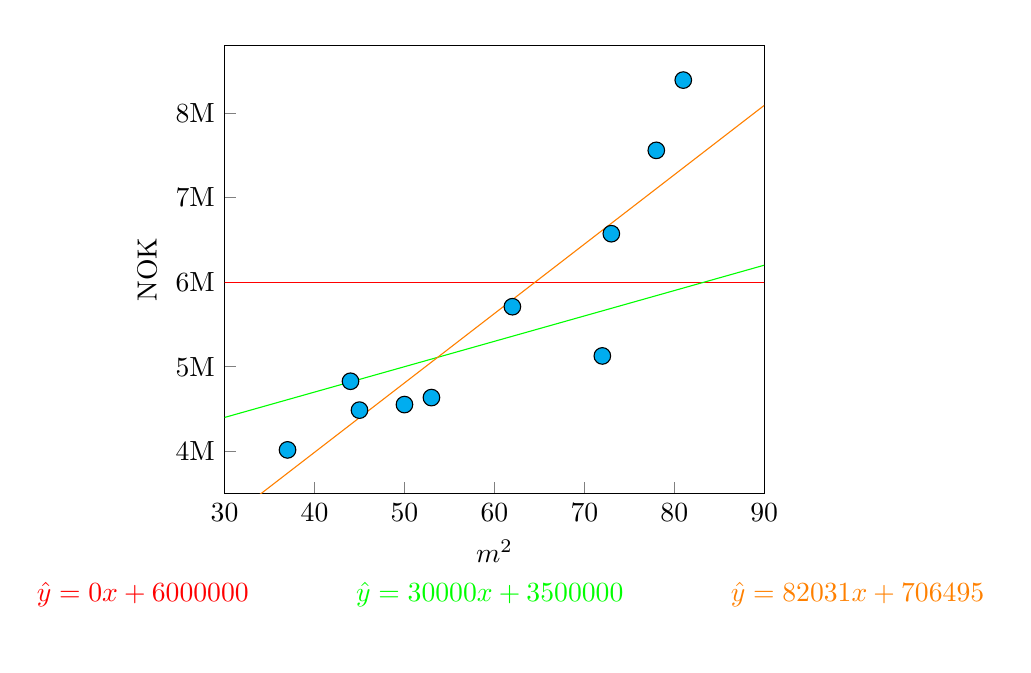
\begin{tikzpicture}
			\begin{axis}[
				xlabel=$m^2$,
				ylabel=NOK,
				ytick={4000000, 5000000, 6000000, 7000000, 8000000},
				yticklabels={4M, 5M, 6M, 7M, 8M},
				scaled y ticks=false,
				xtick pos=bottom,
				ytick pos=left,
				xmin=30,
				xmax=90,,
				ymin=3500000,
				ymax=8800000
			]
				\addplot[
					only marks,
					mark size=3pt,
					mark options={draw=black, fill=cyan}
				] coordinates {
					(72, 5127379)
					(50, 4552170)
					(45, 4486654)
					(62, 5709276)
					(53, 4634912)
					(81, 8388570)
					(44, 4828170)
					(78, 7557770)
					(37, 4016520)
					(73, 6572351)
				};
				\addplot[model1] coordinates {
					(0, 6000000)
					(100, 6000000)
				};
				\addplot[model2] coordinates {
					(0, 3500000)
					(100, 6500000)
				};
				\addplot[model3] coordinates {
					(0, 706495)
					(100, 8909658)
				};

				\newcommand{\loss}[2]{
					\addplot[dashed] coordinates {
						(####1, 3500000 + ####1 * 30000)
						(####1, ####2)
					};
				}

				\coordinate (center) at (axis cs: 60, 3500000);
			\end{axis}
			\node[anchor=north,align=center, text=model2] (m1) at ($ (center) - (0, 1) $) {
				$\hat{y}=30000x + 3500000$
			};

			\node[anchor=east,align=center, text=model1] at ($ (m1.west) + (-1, 0) $) {
				$\hat{y}=0x + 6000000$
			};

			\node[anchor=west,align=center, text=model3] at ($ (m1.east) + (1, 0) $) {
				$\hat{y}=82031x + 706495$
			};

			\node[] at ($ (center) - (5.3, 1.8) $) {};
			\node[] at ($ (center) + (5.3, 5.8) $) {};
		\end{tikzpicture}
		\vfill
	\end{frame}

	\begin{frame}{Loss functions} % Model
		\vfill
		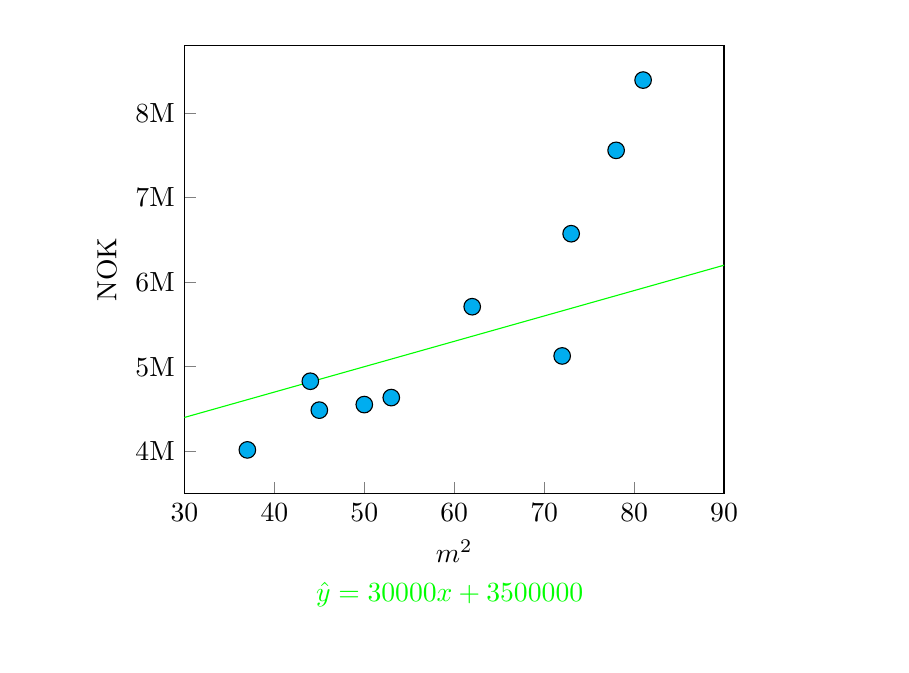
\begin{tikzpicture}
			\begin{axis}[
				xlabel=$m^2$,
				ylabel=NOK,
				ytick={4000000, 5000000, 6000000, 7000000, 8000000},
				yticklabels={4M, 5M, 6M, 7M, 8M},
				scaled y ticks=false,
				xtick pos=bottom,
				ytick pos=left,
				xmin=30,
				xmax=90,,
				ymin=3500000,
				ymax=8800000
			]
				\addplot[
					only marks,
					mark size=3pt,
					mark options={draw=black, fill=cyan}
				] coordinates {
					(72, 5127379)
					(50, 4552170)
					(45, 4486654)
					(62, 5709276)
					(53, 4634912)
					(81, 8388570)
					(44, 4828170)
					(78, 7557770)
					(37, 4016520)
					(73, 6572351)
				};
				\addplot[model2] coordinates {
					(0, 3500000)
					(100, 6500000)
				};

				\newcommand{\loss}[2]{
					\addplot[dashed] coordinates {
						(####1, 3500000 + ####1 * 30000)
						(####1, ####2)
					};
				}

				\coordinate (center) at (axis cs: 60, 3500000);
			\end{axis}
			\node[anchor=north,align=center, text=model2] (m1) at ($ (center) - (0, 1) $) {
				$\hat{y}=30000x + 3500000$
			};

			\node[] at ($ (center) - (5.3, 1.8) $) {};
			\node[] at ($ (center) + (5.3, 5.8) $) {};
		\end{tikzpicture}
		\vfill
	\end{frame}

	\begin{frame}{Loss functions} % Prediction
		\vfill
		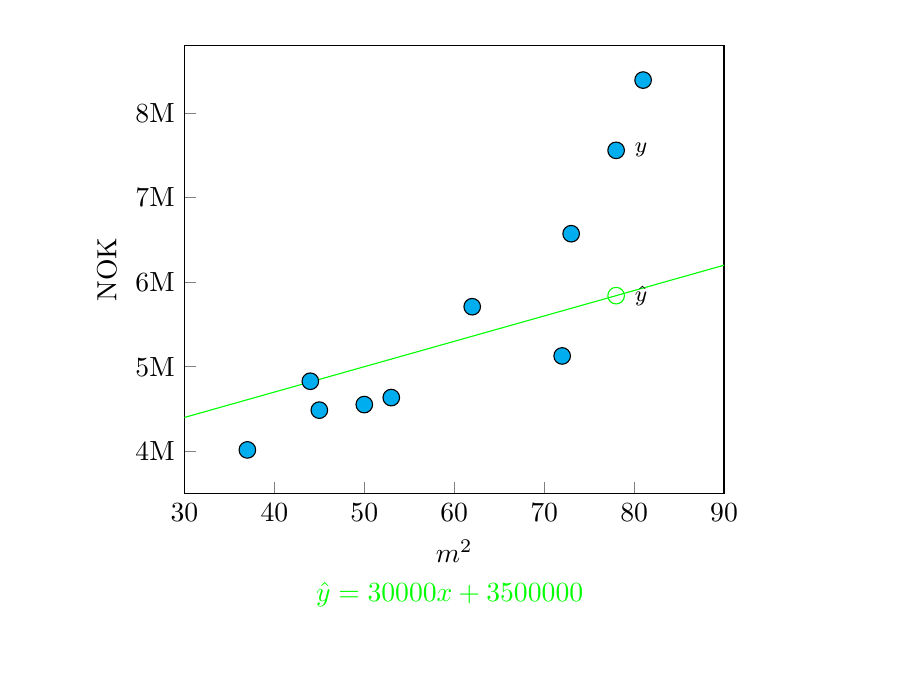
\begin{tikzpicture}
			\begin{axis}[
				xlabel=$m^2$,
				ylabel=NOK,
				ytick={4000000, 5000000, 6000000, 7000000, 8000000},
				yticklabels={4M, 5M, 6M, 7M, 8M},
				scaled y ticks=false,
				xtick pos=bottom,
				ytick pos=left,
				xmin=30,
				xmax=90,,
				ymin=3500000,
				ymax=8800000
			]
				\addplot[
					only marks,
					mark size=3pt,
					mark options={draw=black, fill=cyan}
				] coordinates {
					(72, 5127379)
					(50, 4552170)
					(45, 4486654)
					(62, 5709276)
					(53, 4634912)
					(81, 8388570)
					(44, 4828170)
					(78, 7557770)
					(37, 4016520)
					(73, 6572351)
				};
				\addplot[
					only marks,
					mark size=3pt,
					mark options={draw=green, fill=white},
					fill opacity=0
				] coordinates {
					(78, 3500000 + 78 * 30000)
				};
				\addplot[model2] coordinates {
					(0, 3500000)
					(100, 6500000)
				};

				\newcommand{\loss}[2]{
					\addplot[dashed] coordinates {
						(####1, 3500000 + ####1 * 30000)
						(####1, ####2)
					};
				}

				\coordinate (center) at (axis cs: 60, 3500000);
				\node[anchor=west] at (axis cs: 79, 5840000) {\footnotesize{$\hat{y}$}};
				\node[anchor=west] at (axis cs: 79, 7557770) {\footnotesize{$y$}};
			\end{axis}
			\node[anchor=north,align=center, text=model2] (m1) at ($ (center) - (0, 1) $) {
				$\hat{y}=30000x + 3500000$
			};

			\node[] at ($ (center) - (5.3, 1.8) $) {};
			\node[] at ($ (center) + (5.3, 5.8) $) {};
		\end{tikzpicture}
		\vfill
	\end{frame}

	\begin{frame}{Loss functions} % Squared error
		\vfill
		\begin{tikzpicture}
			\begin{axis}[
				xlabel=$m^2$,
				ylabel=NOK,
				ytick={4000000, 5000000, 6000000, 7000000, 8000000},
				yticklabels={4M, 5M, 6M, 7M, 8M},
				scaled y ticks=false,
				xtick pos=bottom,
				ytick pos=left,
				xmin=30,
				xmax=90,,
				ymin=3500000,
				ymax=8800000
			]
				\addplot[
					only marks,
					mark size=3pt,
					mark options={draw=black, fill=cyan}
				] coordinates {
					(72, 5127379)
					(50, 4552170)
					(45, 4486654)
					(62, 5709276)
					(53, 4634912)
					(81, 8388570)
					(44, 4828170)
					(78, 7557770)
					(37, 4016520)
					(73, 6572351)
				};
				\addplot[
					only marks,
					mark size=3pt,
					mark options={draw=green, fill=white},
					fill opacity=0
				] coordinates {
					(78, 3500000 + 78 * 30000)
				};
				\addplot[model2] coordinates {
					(0, 3500000)
					(100, 6500000)
				};

				\newcommand{\loss}[2]{
					\addplot[dashed] coordinates {
						(####1, 3500000 + ####1 * 30000)
						(####1, ####2)
					};
				}

				\loss{78}{7557770}

				\coordinate (center) at (axis cs: 60, 3500000);
				\node[anchor=west] at (axis cs: 79, 5840000) {\footnotesize{$\hat{y}$}};
				\node[anchor=west] at (axis cs: 79, 7557770) {\footnotesize{$y$}};
				\node[anchor=west] at (axis cs: 78, 6698885) {\footnotesize{$\ell=(y-\hat{y})^2$}};
			\end{axis}
			\node[anchor=north,align=center, text=model2] (m1) at ($ (center) - (0, 1) $) {
				$\hat{y}=30000x + 3500000$
			};

			\node[] at ($ (center) - (5.3, 1.8) $) {};
			\node[] at ($ (center) + (5.3, 5.8) $) {};
		\end{tikzpicture}
		\vfill
	\end{frame}

	\begin{frame}{Loss functions} % Mean squared error
		\vfill
		\begin{tikzpicture}
			\begin{axis}[
				xlabel=$m^2$,
				ylabel=NOK,
				ytick={4000000, 5000000, 6000000, 7000000, 8000000},
				yticklabels={4M, 5M, 6M, 7M, 8M},
				scaled y ticks=false,
				xtick pos=bottom,
				ytick pos=left,
				xmin=30,
				xmax=90,,
				ymin=3500000,
				ymax=8800000
			]
				\addplot[
					only marks,
					mark size=3pt,
					mark options={draw=black, fill=cyan}
				] coordinates {
					(72, 5127379)
					(50, 4552170)
					(45, 4486654)
					(62, 5709276)
					(53, 4634912)
					(81, 8388570)
					(44, 4828170)
					(78, 7557770)
					(37, 4016520)
					(73, 6572351)
				};
				\addplot[
					only marks,
					mark size=3pt,
					mark options={draw=green, fill=white},
					fill opacity=0
				] coordinates {
					(72, 3500000 + 72 * 30000)
					(50, 3500000 + 50 * 30000)
					(45, 3500000 + 45 * 30000)
					(62, 3500000 + 62 * 30000)
					(53, 3500000 + 53 * 30000)
					(81, 3500000 + 81 * 30000)
					(44, 3500000 + 44 * 30000)
					(78, 3500000 + 78 * 30000)
					(37, 3500000 + 37 * 30000)
					(73, 3500000 + 73 * 30000)
				};
				\addplot[model2] coordinates {
					(0, 3500000)
					(100, 6500000)
				};

				\newcommand{\loss}[2]{
					\addplot[dashed] coordinates {
						(####1, 3500000 + ####1 * 30000)
						(####1, ####2)
					};
				}

				\loss{72}{5127379}
				\loss{50}{4552170}
				\loss{45}{4486654}
				\loss{62}{5709276}
				\loss{53}{4634912}
				\loss{81}{8388570}
				\loss{44}{4828170}
				\loss{78}{7557770}
				\loss{37}{4016520}
				\loss{73}{6572351}

				\coordinate (center) at (axis cs: 60, 3500000);
			\end{axis}
			\node[anchor=north,align=center, text=model2] (m1) at ($ (center) - (0, 1) $) {
				$\hat{y}=30000x + 3500000$\\
				$\ell=\sum (y - \hat{y})^2$
			};

			\node[] at ($ (center) - (5.3, 1.8) $) {};
			\node[] at ($ (center) + (5.3, 5.8) $) {};
		\end{tikzpicture}
		\vfill
	\end{frame}

	\begin{frame}{Loss functions} % Loss computation
		\vfill
		\begin{tikzpicture}
			\begin{axis}[
				xlabel=$m^2$,
				ylabel=NOK,
				ytick={4000000, 5000000, 6000000, 7000000, 8000000},
				yticklabels={4M, 5M, 6M, 7M, 8M},
				scaled y ticks=false,
				xtick pos=bottom,
				ytick pos=left,
				xmin=30,
				xmax=90,,
				ymin=3500000,
				ymax=8800000
			]
				\addplot[
					only marks,
					mark size=3pt,
					mark options={draw=black, fill=cyan}
				] coordinates {
					(72, 5127379)
					(50, 4552170)
					(45, 4486654)
					(62, 5709276)
					(53, 4634912)
					(81, 8388570)
					(44, 4828170)
					(78, 7557770)
					(37, 4016520)
					(73, 6572351)
				};
				\addplot[
					only marks,
					mark size=3pt,
					mark options={draw=green, fill=white},
					fill opacity=0
				] coordinates {
					(72, 3500000 + 72 * 30000)
					(50, 3500000 + 50 * 30000)
					(45, 3500000 + 45 * 30000)
					(62, 3500000 + 62 * 30000)
					(53, 3500000 + 53 * 30000)
					(81, 3500000 + 81 * 30000)
					(44, 3500000 + 44 * 30000)
					(78, 3500000 + 78 * 30000)
					(37, 3500000 + 37 * 30000)
					(73, 3500000 + 73 * 30000)
				};
				\addplot[model2] coordinates {
					(0, 3500000)
					(100, 6500000)
				};

				\newcommand{\loss}[2]{
					\addplot[dashed] coordinates {
						(####1, 3500000 + ####1 * 30000)
						(####1, ####2)
					};
				}

				\loss{72}{5127379}
				\loss{50}{4552170}
				\loss{45}{4486654}
				\loss{62}{5709276}
				\loss{53}{4634912}
				\loss{81}{8388570}
				\loss{44}{4828170}
				\loss{78}{7557770}
				\loss{37}{4016520}
				\loss{73}{6572351}

				\coordinate (center) at (axis cs: 60, 3500000);
			\end{axis}
			\node[anchor=north,align=center, text=model2] (m1) at ($ (center) - (0, 1) $) {
				$\hat{y}=30000x + 3500000$\\
				$\ell=1.10 \times 10^{13}$
			};

			\node[] at ($ (center) - (5.3, 1.8) $) {};
			\node[] at ($ (center) + (5.3, 5.8) $) {};
		\end{tikzpicture}
		\vfill
	\end{frame}

	\begin{frame}{Loss functions} % Loss comparison
		\vfill
		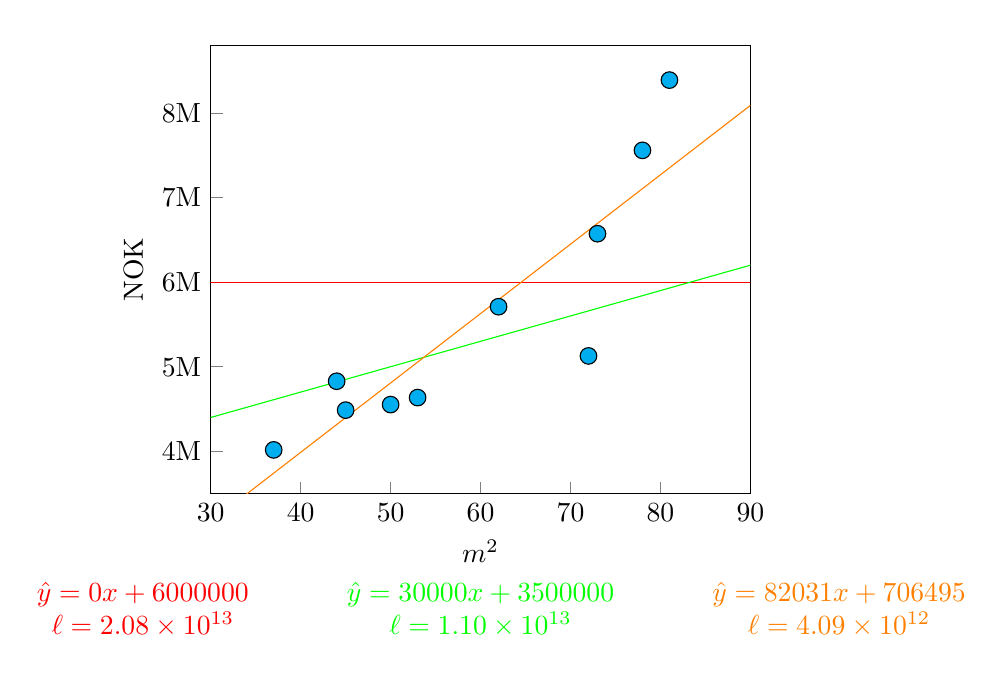
\begin{tikzpicture}
			\begin{axis}[
				xlabel=$m^2$,
				ylabel=NOK,
				ytick={4000000, 5000000, 6000000, 7000000, 8000000},
				yticklabels={4M, 5M, 6M, 7M, 8M},
				scaled y ticks=false,
				xtick pos=bottom,
				ytick pos=left,
				xmin=30,
				xmax=90,,
				ymin=3500000,
				ymax=8800000
			]
				\addplot[
					only marks,
					mark size=3pt,
					mark options={draw=black, fill=cyan}
				] coordinates {
					(72, 5127379)
					(50, 4552170)
					(45, 4486654)
					(62, 5709276)
					(53, 4634912)
					(81, 8388570)
					(44, 4828170)
					(78, 7557770)
					(37, 4016520)
					(73, 6572351)
				};
				\addplot[model1] coordinates {
					(0, 6000000)
					(100, 6000000)
				};
				\addplot[model2] coordinates {
					(0, 3500000)
					(100, 6500000)
				};
				\addplot[model3] coordinates {
					(0, 706495)
					(100, 8909658)
				};
				\coordinate (center) at (axis cs: 60, 3500000);
			\end{axis}
			\node[anchor=north,align=center, text=model2] (m1) at ($ (center) - (0, 1) $) {
				$\hat{y}=30000x + 3500000$\\
				$\ell=1.10 \times 10^{13}$
			};


			\node[anchor=east,align=center, text=model1] at ($ (m1.west) + (-1, 0) $) {
				$\hat{y}=0x + 6000000$\\
				$\ell=2.08 \times 10^{13}$
			};

			\node[anchor=west,align=center, text=model3] at ($ (m1.east) + (1, 0) $) {
				$\hat{y}=82031x + 706495$\\
				$\ell=4.09 \times 10^{12}$
			};

			\node[] at ($ (center) - (5.3, 1.8) $) {};
			\node[] at ($ (center) + (5.3, 5.8) $) {};
		\end{tikzpicture}
		\vfill
	\end{frame}

	\begin{frame}{Loss functions} % Formulas
		\vfill
		\begin{tikzpicture}
			\begin{axis}[
				xlabel=$m^2$,
				ylabel=NOK,
				ytick={4000000, 5000000, 6000000, 7000000, 8000000},
				yticklabels={4M, 5M, 6M, 7M, 8M},
				scaled y ticks=false,
				xtick pos=bottom,
				ytick pos=left,
				xmin=30,
				xmax=90,,
				ymin=3500000,
				ymax=8800000
			]
				\addplot[
					only marks,
					mark size=3pt,
					mark options={draw=black, fill=cyan}
				] coordinates {
					(72, 5127379)
					(50, 4552170)
					(45, 4486654)
					(62, 5709276)
					(53, 4634912)
					(81, 8388570)
					(44, 4828170)
					(78, 7557770)
					(37, 4016520)
					(73, 6572351)
				};
				\addplot[model2] coordinates {
					(0, 3500000)
					(100, 6500000)
				};
				\coordinate (center) at (axis cs: 60, 3500000);
			\end{axis}
			\node[anchor=north,align=center] (m1) at ($ (center) - (0, 1) $) {
				$\hat{y}=Wx + b$\\
				$\ell=\sum (y - \hat{y})^2$
			};

			\node[] at ($ (center) - (5.3, 1.8) $) {};
			\node[] at ($ (center) + (5.3, 5.8) $) {};
		\end{tikzpicture}
		\vfill
	\end{frame}

	\begin{frame}{Loss functions} % Formulas
		\vfill
		\begin{tikzpicture}
			\begin{axis}[
				xlabel=$m^2$,
				ylabel=NOK,
				ytick={4000000, 5000000, 6000000, 7000000, 8000000},
				yticklabels={4M, 5M, 6M, 7M, 8M},
				scaled y ticks=false,
				xtick pos=bottom,
				ytick pos=left,
				xmin=30,
				xmax=90,,
				ymin=3500000,
				ymax=8800000
			]
				\addplot[
					only marks,
					mark size=3pt,
					mark options={draw=black, fill=cyan}
				] coordinates {
					(72, 5127379)
					(50, 4552170)
					(45, 4486654)
					(62, 5709276)
					(53, 4634912)
					(81, 8388570)
					(44, 4828170)
					(78, 7557770)
					(37, 4016520)
					(73, 6572351)
				};
				\addplot[model2] coordinates {
					(0, 3500000)
					(100, 6500000)
				};
				\coordinate (center) at (axis cs: 60, 3500000);
			\end{axis}


			\node[anchor=north,align=center] (m1) at ($ (center) - (0, 1) $) {
				$\hat{y}=Wx + b$\\
				$\ell=\sum (y - \hat{y})^2$
			};
			\node[
				draw=red,
				anchor=north west,
				minimum height=0.4cm,
				minimum width=0.3cm
			] at ($ (m1.north west) + (0.21, -0.03) $) {};
			\node[
				draw=red,
				anchor=south east,
				minimum height=0.4cm,
				minimum width=0.3cm
			] at ($ (m1.south east) + (-0.27, 0.05) $) {};

			\node[] at ($ (center) - (5.3, 1.8) $) {};
			\node[] at ($ (center) + (5.3, 5.8) $) {};
		\end{tikzpicture}
		\vfill
	\end{frame}

	\begin{frame}{Loss functions} % Formulas
		\vfill
		\begin{tikzpicture}
			\begin{axis}[
				xlabel=$m^2$,
				ylabel=NOK,
				ytick={4000000, 5000000, 6000000, 7000000, 8000000},
				yticklabels={4M, 5M, 6M, 7M, 8M},
				scaled y ticks=false,
				xtick pos=bottom,
				ytick pos=left,
				xmin=30,
				xmax=90,,
				ymin=3500000,
				ymax=8800000
			]
				\addplot[
					only marks,
					mark size=3pt,
					mark options={draw=black, fill=cyan}
				] coordinates {
					(72, 5127379)
					(50, 4552170)
					(45, 4486654)
					(62, 5709276)
					(53, 4634912)
					(81, 8388570)
					(44, 4828170)
					(78, 7557770)
					(37, 4016520)
					(73, 6572351)
				};
				\addplot[model2] coordinates {
					(0, 3500000)
					(100, 6500000)
				};
				\coordinate (center) at (axis cs: 60, 3500000);
			\end{axis}


			\node[anchor=north,align=center] (m1) at ($ (center) - (0, 1) $) {
				$\ell=\sum (y - (Wx + b))^2$
			};

			\node[] at ($ (center) - (5.3, 1.8) $) {};
			\node[] at ($ (center) + (5.3, 5.8) $) {};
		\end{tikzpicture}
		\vfill
	\end{frame}

	\begin{frame}{Summary}
		\colorlet{answers}{cyan}
		\vfill
		\begin{itemize}
			\item{What is a statistical learning model?\\
				  \textcolor{answers}{A formula expressing a relationship between inputs and outputs}}
			\item{What is a loss function?\\
				  \textcolor{answers}{A function quantifying how good a set of predictions are}}
			\item{How do we train a statistical learning model?\\
				  \textcolor{answers}{By applying gradual updates of parameters using gradient descent}}
			\item{How does a (deep) neural network work?\\
				  \textcolor{answers}{Sequentially applying (non-linear) artificial neurons to transform inputs}}
			\item{What operations does a convolutional neural network use?\\
				  \textcolor{answers}{Alternating convolutions and pooling, to match patterns in the input}}
			\item{What is transfer learning?\\
				  \textcolor{answers}{Retraining an already trained model for a new problem}}
			\item{What is overfitting?\\
				  \textcolor{answers}{When a model learns patterns in the training data that does not hold generally}}
			\item{How do we combat it?\\
				  \textcolor{answers}{Rigorous testing, regularization and data augmentation}}
		\end{itemize}
		\vfill
	\end{frame}
\end{document}
